\chapter{Protocol Description}
\label{chp:protocol-description}

In this chapter, version 1.0 of the proposed protocol is described in detail, along with assumptions about the environment the protocol will run in, and the intended security goals.


\section{Goals}\label{sec:goals}

The overarching goal of the protocol is to ensure that all parties participating in communication with the satellite can trust that all messages passed through the protocol were sent by another authenticated party. In other words, the satellite should only respond to commands from peers knowing a key to the satellite, and ground stations should be certain that all messages received come from the correct satellite.

The protocol will be based on clients initiating sessions with the satellite, where sessions can last as long as required by the client. Each session is authenticated with a unique session key.

Any of the parties can send an arbitrary amount of messages over a session, and both parties can send messages without any hint from the other party. It is thus possible for a server to send diagnostic data when a session is established, or a list of available actions, without a prior message from the client. This is completely up to the application protocol.

The protocol does not attempt to provide confidentiality, as there's legal restrictions for usage of encryption on ham radio frequencies \cite[article 25.2A, p.~295]{radio-regulations}.

The protocol also does not try to protect against \gls{dos}, as most deployments will be radio-based, and can thus be rendered useless by jamming the frequencies. However, DoS attacks due to resource exhaustion on any of the endpoints will be mitigated where possible.

Fragmentation and re-assembly of data is another non-goal that's delegated somewhere else in protocol stack if desired by the application. The goal is to provide a protocol similar to UDP in characteristics, but with some extra authentication features.


\section{Environment Assumptions}\label{sec:environment_assumptions}

    \subsection{Resource Constrained Server}

As the original problem description involved a satellite with heavy resource constraints, previous attempts at defining a protocol have assumed that public key operations would be too heavy in this environment, and based their authentication on lighter operations such as shared-key MACs. As shown later in this paper, this assumption does not hold for the Raspberry Pis, which can do each of the operations key generation, signing, verification and derive a shared secret, in approximately \( 5 ms \). See \autoref{chp:public-key-raspberry-pi} for more details.

Since the project is aimed at eventually being integrated onto the satellite platform, we have aimed for compatibility with the slower hardware on the actual satellite, and utilized public key cryptography only where strictly necessary, which is the master key re-negotiation phase.

Utilizing public key cryptography would mitigate the need for pre-shared secrets, and would make identity management a bit easier since each session could be identified by the public keys of the partners, instead of lower-layer addresses, but the same considerations regarding replay attacks would have to be taken. It would also be possible to recover from a loss of the private part of the key by simply generating a new pair and broadcasting the new public part, if the clients are willing to trust this new key.

For completeness we'd like to mention that utilizing public key cryptography for signing messages would make it possible for any listening party to verify that message signatures are indeed valid, and do not contain any hidden data. This is in contrast to the MAC-based design, where you'd have to know the secret key to verify the MACs, and two parties could thus claim to follow the protocol, but add hidden data in the MAC field, which would be undetectable by any other listening party.


    \subsection{RNG Reliability}

For the defined protocol to stay secure, a strong \gls{rng} is required on at least one side of the communication, preferably both. Normal computers have access to high-quality random data through either \texttt{/dev/urandom} on most \glspl{*nix} or \texttt{CryptGenRandom} on Windows. The Raspberry Pis have a \gls{hwrng} on-chip, which we assume we can trust, but the satellite does not have such a source. This source is assumed to be present and reliable, but implementation is outside the scope of this paper. For a more in-depth discussion of the \gls{rng}, see \autoref{chp:random-numbers}.


    \subsection{Error-Free Communications Channel}

The protocol assumes that packets sent and received will be error-free, and assumes the underlying layer discards packets with bit errors. In our test setup, UDP will silently discard faulty packets. It's not a problem if the underlying layer doesn't detect errors, as that will be caught in the MAC check, the only benefit of detecting it on a lower layer is if there's an interest to doing \gls{arq} to improve reliability, as NAP will drop all faulty messages without any feedback to the client.


    \subsection{Broadcast Channel}

We assume that there might be several clients and several servers communicating over the same frequencies, and that they're all in range of each other, everyone hearing all messages. This assumption is stronger than for previous projects, and introduces the demand for authentication of both sides of the communication. Previous projects were targeted directly to NUTS, in which you'd have a slightly stronger argument that the signals you're receiving actually come from the satellite as they match the satellites latency, doppler shift and position, but these are not trustworthy indicators to cryptographers. Nor do they apply in other environments where you don't have these very directional antennas, like in our test environment.


\section{The Protocol}\label{sec:the_protocol}

\begin{figure}[ht!]
\centering
\includegraphics[width=120mm]{protocol-packet-flow}
\caption{Packet flows in the protocol. \( R_a \) and \( R_b \) are nonces generated by the server and client, respectively. \( N_s \) and \( N_c \) are monotonically increasing sequence numbers, to keep each packet (and by extension, MAC) unique. Both parties possess the shared key \( K \), and use the nonces to derive a session key \( S \) after a mutual challenge-response handshake.}\label{fig:protocol-packet-flow}
\end{figure}

Here follows an overview of the different messages sent back and forth in the \acrfull{nap}. All messages follow a general format, as seen in \autoref{tab:general-packet-structure}. The most important messages and their cryptographic parameters are show in the sequence diagram in \autoref{fig:protocol-packet-flow}.

\begin{table}[ht!]
\centering
    \begin{tabular}{r | c | c | c | c |}
    \cline{2-5}
    Byte range & 0--1 & 1--2 & 2--(n-mac\_len) & (n-mac\_len)--n \\ \cline{2-5}
    Content & Type & Sequence number & Application data & MAC \\ \cline{2-5}
    \end{tabular}
    \caption{General packet structure for packet of length \( n \). Sequence numbers are not present on handshake messages. We assume for simplicity here that the sequence number can be represented as a single byte.}\label{tab:general-packet-structure}
\end{table}

The MAC field is generally computed as \( MAC_{key}(MSG\_TYPE \| MSG \ [\| OPTIONS]) \), where the key is either the shared secret \( K \) in the case of the first handshake messages, or the session key \( S \) in the case of the others. OPTIONS are used in the handshake phase to respond to challenges issued by communicating parties, which is not part of the reply. A more thorough description of all the different messages is given below.


    \subsection{The Session Key}\label{sec:session-key}

The session key \gls{kdf} used for \gls{nap} is \gls{hkdf} \cite{hkdf}, as standardized through RFC 5869 \cite{rfc5869}. The \gls{hkdf} computation involves two phases using HMAC-SHA512; key material extraction and then key expansion, with the parameters as shown in \autoref{eq:hkdf}.

\begin{equation}
    \begin{aligned}
    pseudo\_random\_key& = extract(salt, input\_keying\_material) \\
    key& = expand(pseduo\_random\_key, info, length=32)
    \end{aligned}
    \label{eq:hkdf}
\end{equation}

NAP uses the values defined in \autoref{tab:hkdf-parameters} for the different parameters.

\begin{table}[ht!]
\centering
    \begin{tabular}{| l | l |}
    \hline
    \textbf{Parameter} & \textbf{Value} \\ \hline
    input\_keying\_material & shared secret \\ \hline
    salt & \( R_a \| R_b \) \\ \hline
    info & protocol version (e.g. "1.0") \\ \hline
    length & 16 \\ \hline
    \end{tabular}
    \caption{HKDF parameter values for session key generation}\label{tab:hkdf-parameters}
\end{table}


    \subsection{Protocol Messages}\label{subsec:protocol-messages}

Here we'll take a more detailed look at the different messages. Each message sent starts with a byte indicating the type of message, optionally some more parameters, some content, and a MAC, as illustrated in \autoref{tab:general-packet-structure}. The starting byte of the message also indicates which side of the protocol issued the message, thus preventing duplicate MACs even if the content in a message from the server is identical to that of one from the client and the sequence numbers sync up. The bytes assigned to each message can be seen in \autoref{tab:protocol-messages}.

\begin{table}
\caption{Protocol messages in NAP}\label{tab:protocol-messages}
\centering
    \begin{tabular}{| l | l | p{5cm} |}
    \hline
    \textbf{Byte} & \textbf{Symbolic name} & \textbf{Description} \\ \hline
    0x00 & CLIENT\_HELLO & First message from client, with challenge to server and protocol version \\ \hline
    0x01 & SA\_PROPOSAL & Security association suggested by client \\ \hline
    0x02 & CLIENT\_DATA & Application data from the client \\ \hline
    0x03 & REKEY & Negotiate a new master secret \\ \hline
    0x04 & REKEY\_CONFIRM & Commit the new shared master key \\ \hline
    0x05--0x07e & Unassigned & \\ \hline
    0x7f & CLIENT\_TERMINATE & Client is terminating the session \\ \hline
    0x80 & SERVER\_HELLO & First response from server, responds to client challenge and challenges client \\ \hline
    0x81 & SA & Negotiated security association from server \\ \hline
    0x82 & SERVER\_DATA & Application data from the server \\ \hline
    0x83 & VERSION\_NOT\_SUPPORTED & Version suggested by client is not supported by server \\ \hline
    0x84 & REKEY\_RESPONSE & Respond to a re-key request by sending the server's public key \\ \hline
    0x85 & REKEY\_COMPLETED & Confirm back to the client that the re-keying has been committed \\ \hline
    0x86--0x8e & Unassigned & \\ \hline
    0xff & SERVER\_TERMINATE & Server is terminating the session \\ \hline
    \end{tabular}
\end{table}

There's plenty of room for expansion in the protocol, either for future standard types defined in upcoming versions or for extensions to utilize. Note that these message types are only for NAP, application-level protocols should define their own message format and use that to differentiate the different kinds of messages that might come through.

The maximum message size supported by the protocol is a function of the \gls{mtu} of the underlying transport. The protocol therefore exposes it's MTU to the application, which is defined as \( MTU_{NAP} = MTU_{T} - (5 + mac\_len) \), where the overhead added by a session is the sum of it's MAC length, the type byte and up to 4 bytes of sequence number. It's up to the application-layer protocol to perform fragmentation and re-assembly if it requires support for messages larger than the MTU of the NAP session.


        \subsubsection{CLIENT\_HELLO}

\begin{table}[ht!]
\centering
    \begin{tabular}{r | c | c | c | c |}
    \cline{2-5}
    Byte range & 0--1 & 1--2 & 2--10 & 10--18 \\ \cline{2-5}
    Content & 0x00 & Version & \( R_b \) & MAC \\ \cline{2-5}
    \end{tabular}
    \caption{Packet structure of CLIENT\_HELLO packets. Total size: 18 bytes.}
\end{table}

The first message exchanged in a session is the CLIENT\_HELLO. The version is the highest version of the protocol the client supports. The client generates a random number \( R_b \), computes the MAC as \( MAC_k(0x00 \| Version \| R_b ) \), and sends it to the master. \( R_b \) serves as a challenge to the master, to make sure we're talking to someone that legitimately knows the shared secret.

The version supported should be encoded as a single byte, with the four major bits indicating the major version, and the lower four bits indicating the minor version. 0x10 thus represents version 1.0, while 0xff is the highest supported version of 15.15. This is hopefully enough to allow the protocol to grow for quite some time.


        \subsubsection{SERVER\_HELLO}

\begin{table}[ht!]
\centering
    \begin{tabular}{r | c | c | c |}
    \cline{2-4}
    Byte range & 0--1 & 1--(n-8) & (n-8)--n \\ \cline{2-4}
    Content & 0x80 & \( R_a \) & MAC \\ \cline{2-4}
    \end{tabular}
    \caption{Packet structure of SERVER\_HELLO packets. Total size: 17 bytes.}
\end{table}

The SERVER\_HELLO is the first message from the server, sent in response to a CLIENT\_HELLO. The messages answers the client's challenge and thus proves the identity of the server, and provides a challenge to the client. Receiving this message instead of a VERSION\_NOT\_SUPPORTED also means that the server supports the version suggested by the client.

The server needs to generate an 8-byte \( R_a \) and send as a challenge to the client. The MAC is computed as \( MAC_k(0x80 \| R_a \| R_b) \).


        \subsubsection{VERSION\_NOT\_SUPPORTED}

\begin{table}[ht!]
\centering
    \begin{tabular}{r | c | c | c |}
    \cline{2-4}
    Byte range & 0--1 & 1--2 & 2--10 \\ \cline{2-4}
    Content & 0x83 & Highest version supported by server & MAC \\ \cline{2-4}
    \end{tabular}
    \caption{Packet structure of VERSION\_NOT\_SUPPORTED packets. Total size: 10 bytes.}
\end{table}

The VERSION\_NOT\_SUPPORTED message is sent by the server to the client if the protocol version given by the client in the CLIENT\_HELLO is not supported by the server. The message only contains the highest version of the protocol supported by the server. The presence of this message is necessary to prevent version rollback attacks, since if the server simply discarded unknown protocol versions, an attacker could delete all CLIENT\_HELLO messages with a strong version, thus forcing the client to re-try with a weaker version. With the presence of this message, the client can differentiate the cases where a version is unsupported, and messages are lost, and hence will not re-try with weaker versions if the first attempt doesn't generate a response.

The MAC is computed as \( MAC_k(0x83 \| version \| R_b) \). The version should be encoded using the same single-byte encoding as in the CLIENT\_HELLO.

If the client supports the version given by the server it should retry the CLIENT\_HELLO with that version.


        \subsubsection{SA\_PROPOSAL}

\begin{table}[ht!]
\centering
    \begin{tabular}{r | c | c | c |}
    \cline{2-4}
    Byte range & 0--1 & 1--(n-8) & (n-8)--n \\ \cline{2-4}
    Content & 0x01 & CBOR-encoded key-value map & MAC \\ \cline{2-4}
    \end{tabular}
    \caption{Packet structure of SA\_PROPOSAL packets. Total size: From 9 to \gls{mtunap} bytes.}
\end{table}


The \gls{sa} proposal is suggested cryptographic parameters to use for the session, and responds to the challenge from the server. A compliant server should select the union of it's own supported ciphers and the ones suggested by the client, and pick the strongest one. The client can also suggest a length to use for the MAC, which should be a number of bytes between 4 and 32. The SA\_PROPOSAL is sent as a serialized key-value mapping, serialized using \gls{cbor} \cite{cbor}, a compact binary JSON-like serialization format recently standardized by the IETF.

All parameters in the SA has sensible defaults (for the NUTS project), thus usually the client can simply submit an empty proposal, and the server will select the defaults.

\begin{table}
\centering
    \begin{tabular}{| l | l | l |}
    \hline
    Key & Type & Default \\ \hline
    mac & List of suggested MAC algorithms & sha3\_256 \\ \hline
    mac\_len & Integer in the range 4--32 & 8 \\ \hline
    \end{tabular}
    \caption{Potential parameters in the security association suggested by the client.}\label{tab:sa}
\end{table}

The current suggested protocol does not attempt to be overly compact, simply utilizing plain-text names for the protocols to use, and the keys in the mapping. This is done for readability and keeping the scope of the project manageable. If seriously bandwidth constrained a mapping between bytes and MAC algorithms could be made (and probably standardized by IANA), and a similar mapping between keys and their human readable name.

Since this is simply a key-value mapping, extending the protocol with optional parameters for encryption, extensions, timeout values, or anything else should be a simple matter.

The MAC should be computed as \( MAC_k(0x01 \| CBOR-data \| R_a) \), thus answering the challenge from the server and proving knowledge of the shared key.

An implementation of the protocol only has to support Keccak-256, supporting other MACs like HMAC-SHA256 or Keccak-512 is optional.


        \subsubsection{SA}

\begin{table}[ht!]
\centering
    \begin{tabular}{r | c | c | c |}
    \cline{2-4}
    Byte range & 0--1 & 1--(n-8) & (n-8)--n \\ \cline{2-4}
    Content & 0x81 & CBOR-encoded key-value map & MAC \\ \cline{2-4}
    \end{tabular}
    \caption{Packet structure of SA packets. Total size around 30 bytes.}
\end{table}

The \gls{sa} message from the server is the final set of parameters to use for the rest of the session. It contains the MAC algorithm and the length to use as decided by the server. To minimize ambiguity, the parameters are always sent even if just the defaults was selected. The message thus have to include at least the \texttt{mac} and \texttt{mac\_len} keys in the CBOR-encoded key-value mapping.

The MAC for this message is computed using the session key, which is derived using HKDF as described in \autoref{sec:session-key}. The length is still truncated to 8 bytes like all the other handshake messages, since the client can't extract the SA parameters from this message to determine the length before it has validated the MAC.

The size of this message depends on the textual representation of the MAC algorithm selected, and whether any extensions are used. The CBOR encoding of the key-value map for the default parameters will look like this (23 bytes):

\begin{table}[ht!]
\centering
    \begin{tabular}{c | c | c | c | c | c | c | c}
    0xa2 & 0x63 & mac & 0x68 & sha3\_256 & 0x67 & mac\_len & 0x08
    \end{tabular}
\end{table}

The first 0xa2 byte indicates a map with two values, 0x60--0x77 indicates a UTF-8 string of length 0--23, and 0x08 the integer 8. We see that the textual representation of Keccak-256 is 8 bytes, and the only part of this message likely to change much. This is also probably the shortest algorithm to be represented, as "HMAC-SHA1", "HMAC-SHA256", "sha3\_512" and the likes are all as long or longer.


        \subsubsection{CLIENT\_DATA and SERVER\_DATA}

\begin{table}[ht!]
\centering
    \begin{tabular}{r | c | c | c | c |}
    \cline{2-5}
    Byte range & 0--1 & 1--2 & 2--(n-mac\_len) & (n-mac\_len)--n \\ \cline{2-5}
    Content & 0x02/0x82 & Sequence number & Application data & MAC \\ \cline{2-5}
    \end{tabular}
    \caption{Packet structure of CLIENT\_DATA and SERVER\_DATA packets. We assume that the sequence number fits in a single byte in the figure. Total size: at least \( mac\_len+2 \) bytes.}
\end{table}

For CLIENT\_DATA and SERVER\_DATA messages, there is a field for sequence numbers. This is a an integer, encoded as a variable length quantity, meaning sequence numbers will never repeat in a single session, and can grow arbitrarily large. The encoding uses only one byte for all numbers below 127, which is probably sufficient for most sessions. Numbers between 128 and 16383 uses 2 bytes, 16834 to 2097152 uses 3 bytes, and so on. The encoding is the same as the one first used in the MIDI format, using the MSB of each byte to indicate whether there are more bytes following, thus utilizing 7 bits of each byte for the actual number. For practical considerations the maximum length for the sequence number can be limited to 4 bytes to not overflow a 32-bit integer, enabling a maximum of \( 2^{(7 \times 4)} - 1 = 268 435 455 \) messages in a session, or roughly one message per second for 8 consecutive years until you'd have to start a new session.

The MAC for these messages are computed with the session key over the entire message sent.


        \subsubsection{REKEY}

\begin{table}[ht!]
\centering
    \begin{tabular}{r | c | c | c | c |}
    \cline{2-5}
    Byte range & 0--1 & 1--2 & 2--34 & 34--n \\ \cline{2-5}
    Content & 0x03 & Sequence number & Client\_pubkey & MAC \\ \cline{2-5}
    \end{tabular}
    \caption{Packet structure of a REKEY packet. Sequence number is assumed to fit in a single byte for simplicity in this diagram. Total size: \( 34 + mac\_len \) bytes.}
\end{table}

Re-keying is done if the master key is lost or suspected compromised, and is largely equivalent to you losing the password to your email account -- you better be faster than the attacker in changing passwords, or you'll have lost your account. The same goes for the satellite, if the attacker is able to re-key the satellite, you'll be locked out with no hope of getting it back.

Re-keying works by establishing a normal session with the existing key, and then issuing a REKEY message. The REKEY message consist of an ad-hoc Curve25519 public key, and the satellite will respond with it's ad hoc Curve25519 public key. Both parties can now derive the new master key by doing a scalar multiplication of their own private key and the other party's public key. A final pair of messages is exchanged to make sure both parties did indeed arrive at the same new key, and commit the action. For the satellite, this means invalidating all existing sessions, since the compromise of the old master key means all existing sessions can be hijacked, due to the session key being derived from the master key and the two nonces, all of which are now known by the attacker.

Curve25519 is a specification of a an Edwards curve, which can be used in an elliptic curve variant of Diffie-Hellman, which was chosen for it's speed and small size of keys. Public and private keys are both 32 bytes, and the result of the scalar multiplication of the other parties public key and your own private key will be the shared secret, which is also 32 bytes. Following the recommendations from NIST for key establishment (\cite{sp800-56a}), we'll derive the new shared keying material from this shared secret, using the same HKDF construction as used in the handshake, but with different parameters. The parameter used are depicted in \autoref{tab:hkdf-rekey-parameters}.

\begin{table}[ht!]
\centering
    \begin{tabular}{| l | l |}
    \hline
    \textbf{Parameter} & \textbf{Value} \\ \hline
    input\_keying\_material & master key || session key \\ \hline
    salt & shared secret \\ \hline
    info & protocol version (e.g. "1.0") \\ \hline
    length & 32 \\ \hline
    \end{tabular}
    \caption{HKDF parameter values when generating new master secret}\label{tab:hkdf-rekey-parameters}
\end{table}

Since this operation involves public key cryptography, a note about performance is necessary. On the Raspberry Pi, using the \texttt{libsodium} library's implementation of Curve25519 we were able to perform key generation and the scalar multiplication in about \( 8 ms \), which is more than fast enough for our needs. In comparison, generating a single RSA key takes several seconds on the Raspberry Pi. This vastly superior performance is the prime motivation for elliptic curve based operations in general, and the Curve25519 specification and the \texttt{libsodium} implementations in particular. A more detailed benchmark is included in \autoref{chp:public-key-raspberry-pi}.


        \subsubsection{REKEY\_RESPONSE}

\begin{table}[ht!]
\centering
    \begin{tabular}{r | c | c | c | c |}
    \cline{2-5}
    Byte range & 0--1 & 1--2 & 2--34 & 34--n \\ \cline{2-5}
    Content & 0x84 & Sequence number & Server\_pubkey & MAC \\ \cline{2-5}
    \end{tabular}
    \caption{Packet structure of a REKEY\_RESPONSE packet. Sequence number is assumed to fit in a single byte for simplicity in this diagram. Total size: \( 34 + mac\_len \) bytes.}
\end{table}

The REKEY\_RESPONSE is the server replying to a re-key request, with its own ad-hoc Curve25519 public key. Upon receiving the REKEY message and having generated a new keypair, the server has all the components necessary to derive the new master key. It must however wait for the REKEY\_CONFIRM before performing the actual update of the new master key.


        \subsubsection{REKEY\_CONFIRM}

\begin{table}[ht!]
\centering
    \begin{tabular}{r | c | c | c |}
    \cline{2-4}
    Byte range & 0--1 & 1--2 & 2--n \\ \cline{2-4}
    Content & 0x04 & Sequence number & MAC \\ \cline{2-4}
    \end{tabular}
    \caption{Packet structure of a REKEY\_CONFIRM packet. Total size: \( 2 + mac\_len \) bytes.}
\end{table}

The REKEY\_CONFIRM serves to verify that the client and the server have negotiated the same new master key. This message is empty except for the type byte, sequence number and the MAC.

The MAC should be computed with the new master key computed using HKDF as described in the REKEY packet description.

The sequence number doesn't serve a particular purpose in preventing replays for this packet, as replaying this packet doesn't make sense anyway, but it's present to maintain consistency in the sense that every packet exchanged between the parties increases the sequence number.


        \subsubsection{REKEY\_COMPLETED}

\begin{table}[ht!]
\centering
    \begin{tabular}{r | c | c | c |}
    \cline{2-4}
    Byte range & 0--1 & 1--2 & 2--n \\ \cline{2-4}
    Content & 0x85 & Sequence number & MAC \\ \cline{2-4}
    \end{tabular}
    \caption{Packet structure of a REKEY\_CONFIRM packet. Total size: \( 22 + mac\_len \) bytes.}
\end{table}

The REKEY\_COMPLETED confirms to the client that the requested re-key operation has been completed, and a new session can be set up with the newly derived master key. The current session will be terminated, since the parties need to negotiate a new session key, but implementations are free to hide this termination and re-establishment phase from the consumer.


        \subsubsection{CLIENT\_TERMINATE}

\begin{table}[ht!]
\centering
    \begin{tabular}{r | c | c | c |}
    \cline{2-4}
    Byte range & 0--1 & 1--2 & 2--n \\ \cline{2-4}
    Content & 0x7f & Sequence number & MAC \\ \cline{2-4}
    \end{tabular}
    \caption{Packet structure of a CLIENT\_TERMINATE packet. Total size: \( mac\_len + 2 \) bytes.}
\end{table}

The CLIENT\_TERMINATE and SERVER\_TERMINATE messages are sent to indicate that the session is over. In general it would be the client that terminates the session, and it can expect to get a SERVER\_TERMINATE in return to confirm that the session has been deleted on the server.


        \subsubsection{SERVER\_TERMINATE}

\begin{table}[ht!]
\centering
    \begin{tabular}{r | c | c | c | c |}
    \cline{2-5}
    Byte range & 0--1 & 1--2 & 2--3 & 3--n \\ \cline{2-5}
    Content & 0xff & Sequence number & Reason & MAC \\ \cline{2-5}
    \end{tabular}
    \caption{Packet structure of a SERVER\_TERMINATE packet. Total size: \( mac\_len + 3 \) bytes.}
\end{table}

A SERVER\_TERMINATE is generally sent as a confirmation to a termination request from a client, but can also be sent by the server to let the client know it's session has been terminated.

The server might terminate the session if another session has performed a re-key, to let this session know that it's no use trying to continue with this session key. The client thus has to re-establish a new session to continue communication. The server might also terminate the session if it times out. The cause of the termination is sent as the reason, which is a single byte identifying these different cases, as given in \autoref{tab:terminate-reasons}.

\begin{table}[ht!]
\centering
    \begin{tabular}{| c | c |}
    \hline
    \textbf{Byte} & \textbf{Reason} \\ \hline
    0x00 & Client terminated \\ \hline
    0x01 & Re-keyed \\ \hline
    0x02 & Timed out \\ \hline
    \end{tabular}
    \caption{Different reasons given by the server for terminating a session}\label{tab:terminate-reasons}
\end{table}

The client is not expected to reply to a SERVER\_TERMINATE.


    \subsection{Message fragmenting and re-assembly}

NAP does not handle message fragmenting and re-assembly. If the underlying transport protocol has an \gls{mtu}, NAP implementations will have to be aware of this, and should raise an error condition if messages larger than the MTU is attempted sent on the channel. If the application needs to send messages larger than the underlying MTU, it needs to handle fragmentation itself. An example of how this is done is provided in one of the experiments in \autoref{chp:experiments}. Note that if this is the case, it's probably best to use RDP as the underlying transport.


\section{Formal analysis}\label{sec:formal_analysis}

To verify that our protocol adheres to certain security claims, we model it using \gls{spdl} and run it through the \gls{scyther} tool developed by Cas Cremers \cite{scyther}. The most important claim is that our protocol inhibits the non-injective property, which ensures that all messages accepted by either of the parties were accepted in the same order as in the model. This excludes an attacker from re-ordering messages sent, re-routing them to another pair of communicating parties, etc. We also claim that the derived session key will remain known only to the parties with the shared secret. The complete \gls{spdl} can be found in \autoref{chp:nuts-spdl}. Some notes to the model follow.

\gls{scyther} does not have a way to model arbitrary amounts of messages, such as repeated commands in a single session. If only the session establishment is modeled, \gls{scyther} will not be able to detect weaknesses in the rest of the protocol, such as replay attacks for command messages. To circumvent this limitation, we first model an execution of the protocol without sequence numbers (code found in \autoref{chp:nuts-spdl}), to make sure that Scyther detects the replay attack. The resulting attack graph can be seen in \autoref{fig:scyther-replay-attack}.

\begin{figure}[ht!]
\centering
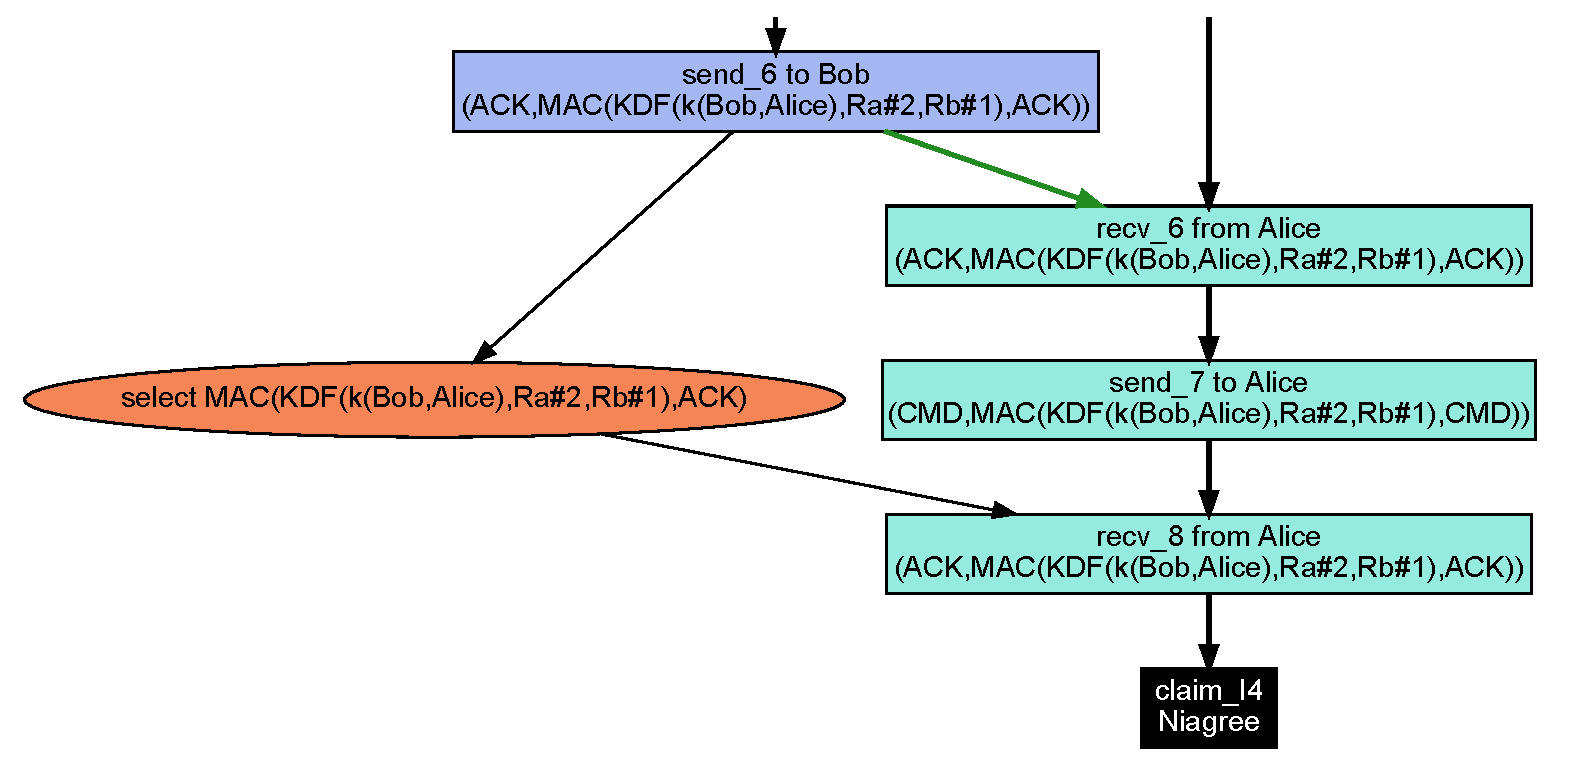
\includegraphics[width=110mm]{auth-without-seqnums}
\caption{Scyther attack graph against NAP without sequence numbers. We see that the attacker (the circle on the left) can extract the first message and send it to to Alice on the right, thus breaking the non-injective agreement.}\label{fig:scyther-replay-attack}
\end{figure}

As we now have a realistic model of how the protocol would work without sequence numbers, we can add sequence numbers to the model, and Scyther is now unable to detect any further attacks on the protocol. We then conclude that the sequence number successfully mitigate the replay attacks, if implemented correctly.

Attempts were made at modeling the re-key operations as well, but due to limitations in Scyther -- particularly no good way to model the scalar multiplication to derive a shared secret -- getting a working model would require too many hacks to simulate this operation to actually prove anything of value.


\section{Sessions}

Sessions in NAP assumes that the underlying layer provides some sort of address that can be used to associate a session to it's state and key. A session can be fully defined by it's state, the address of the other party (size depends on the underlying layer, for IPv4 this is 6 bytes for address and port) and the 16-byte session key, which amounts to a mere 23 bytes of storage.


    \subsection{Session States}

The lifetime of a \gls{session} is accurately described by a \gls{fsm}. A \gls{fsm} model of a NAP session on server side can be seen in \autoref{fig:nap-session-server}.

\begin{figure}[ht!]
\centering
    \digraph[scale=0.5]{sessionstatesserver}{
        rankdir=BT;

        inactive [label="Inactive"];
        wait_for_sa_proposal [label="Wait for SA_PROPOSAL"];
        established [label="Session established"];
        rekey [label="Re-key"];
        hidden [style=invis];

        hidden -> inactive;
        inactive -> wait_for_sa_proposal [label="CLIENT_HELLO"];
        wait_for_sa_proposal -> established [label="SA_PROPOSAL"];
        wait_for_sa_proposal -> inactive [label="Timeout", style=dotted];
        established -> established [label="CLIENT_DATA"]
        established -> inactive [label="CLIENT_TERMINATE"];
        established -> rekey [label="REKEY"];
        established -> inactive [label="Timeout", style=dotted];
        rekey -> inactive [label="REKEY_CONFIRM"];
        rekey -> established [label="Timeout", style=dotted];
    }
    \caption{Finite state machine of a server-side NAP session. In all transitions the MAC is verified, faulty messages are silently discarded. Outgoing messages are not shown.}\label{fig:nap-session-server}
\end{figure}

This model also introduces some considerations not described by the formal analysis in the previous section, most notably the timers. Having timers to automatically demote sessions from active status on inactivity is essential to avoid \gls{dos} due to resource exhaustion. Without this counter-measure, it would be trivial to capture valid \(R_b\) and \(MAC_{k}(R_b)\) pairs sent over the network, and replay them all at the same time to deplete the satellite for memory and/or storage, since it'll have to generate new \(R_a\) pairs for each connecting client. This would be roughly equivalent to the traditional SYN flood attack towards servers running \gls{tcp}\cite{syn_flood}.

Timers also protect the server against non-compliant clients not properly closing sessions, to avoid similar resource depletion. Connection timers is the satellites way to make sure that even when faced with misbehaving clients, resources are properly managed and handled. These problems could also occur due to natural causes, such as no messages coming through due to lots of noise on the radio network, or the satellite orbiting out of a reachable window. Proper resource management makes sure that the satellite can stay operational even after longer periods of time with these sorts of events happening regularly.

The corresponding FSM for a client-side session is shown in \autoref{fig:nap-session-client}.

\begin{figure}[ht!]
\centering
    \digraph[scale=0.45]{sessionstatesclient}{
        rankdir=BT;

        wait_for_server_hello [label="Wait for SERVER_HELLO"];
        wait_for_sa [label="Wait for SA"];
        established [label="Established"];
        wait_for_rekey_response [label="Wait for REKEY_RESPONSE"];
        wait_for_rekey_complete [label="Wait for REKEY_COMPLETE"];
        hidden [style=invis];

        hidden -> wait_for_server_hello [label="Sends CLIENT_HELLO"];
        wait_for_server_hello -> wait_for_sa [label="SERVER_HELLO"];
        wait_for_server_hello -> terminated [label="Timeout", style=dotted];
        wait_for_server_hello -> wait_for_server_hello [label="VERSION_NOT_SUPPORTED"];
        wait_for_sa -> established [label="SA"];
        wait_for_sa -> terminated [label="Timeout", style=dotted];
        established -> wait_for_rekey_response [label="Sends REKEY"];
        established -> established [label="SERVER_DATA"];
        established -> terminated [label="Any party terminates"];
        established -> terminated [label="Timeout", style=dotted];
        wait_for_rekey_response -> wait_for_rekey_complete [label="REKEY_RESPONSE"];
        wait_for_rekey_response -> established [label="Timeout", style=dotted];
        wait_for_rekey_complete -> terminated [label="REKEY_COMPLETE"];
        wait_for_rekey_complete -> established [label="Timeout", style=dotted];

        {rank=same; wait_for_server_hello; hidden; }
    }
    \caption{Finite state machine of a client-side NAP session. In all transitions the MAC is verified, faulty messages are silently discarded. Re-transmissions and failure handling is not shown.}\label{fig:nap-session-client}
\end{figure}

It's also worth noting that incoming packets with invalid \gls{mac} are simply ignored on both sides, and can never cause a session to respond, terminate or change state. This is essential as it's trivial to generate packets with a given source address and invalid \gls{mac} and inject into the communications channel. Allowing them to affect session state would thus be very bad practice, and open up an attack vector of very easy \gls{dos}.


\section{Extension Points}\label{sec:extension-points}

Since the parties can potentially negotiate extensions in the handshake, and there's a bunch of free messages type that extensions can use, there's plenty of opportunities for extending the protocol with whatever features are desired. Some of these are suggested below. Note that these are just suggestions, and are neither included in the sample implementation, nor standardized.


    \subsection{Session Compression Negotiation}

Depending on the deployment, it might make sense to enable support for message compression in the transport layer, similar to what TLS provides. Since the protocol doesn't provide confidentiality, there's no risk for a CRIME-style compromise of cleartext when combining compression and encryption. If implemented this should be configurable, since for some deployments another layer might already provide compression, and transport layer compression would just waste CPU cycles (like sharing JPEG images).


    \subsection{Role-Based Access Control}

For students or other people outside the core NUTS team to be able to use the satellite, to take images of stuff they want or shoot time-lapse videos or similar, a \gls{rbac} system could be implemented, to be able to give them access to certain parts of the satellite, but not others. The system should ideally work on both NAP messages, limiting access to i.e. re-keying, and application specific functions, like being able to take pictures and time-lapse videos, but not upload new code or change orientation.

The motivation for implementing this on the transport layer is that with the absence of confidentiality, passwords or access codes can't be sent in the clear, and application layer developers would have to be familiar with cryptography to be able to develop methods for doing these operations safely. Adding this functionality on the transport layer limits the number of places code that needs auditing resides, and removes the need for application layer cryptographic operations.
